
\begin{frame}
  \frametitle{Computational Methods}
  \begin{figure}[h!]
    \centering
    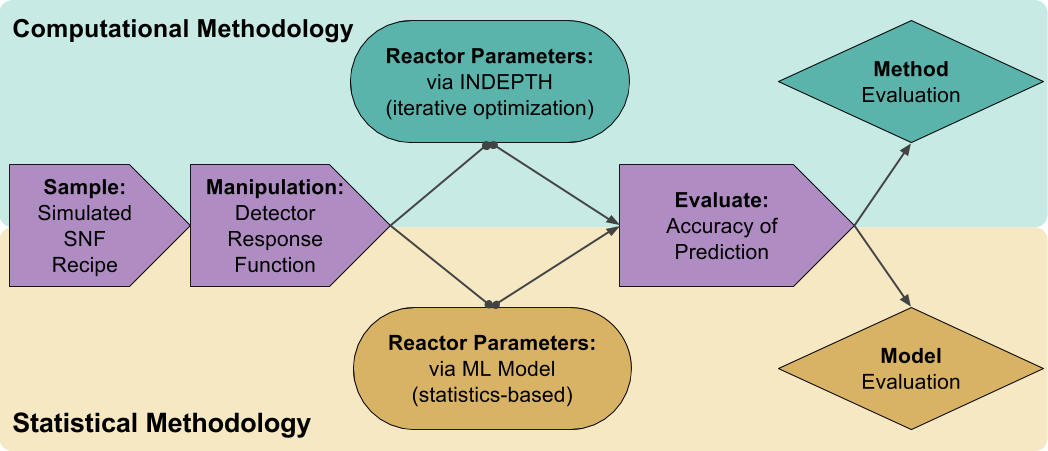
\includegraphics[width=0.9\textwidth]{./figures/CompStatForensicsWorkflow.png}
    \caption{Nuclear forensics research: physical, experimental, and computational}
  \end{figure}
\end{frame}

\begin{frame}
  \frametitle{Computational Methods}
  \begin{figure}[h!]
    \centering
    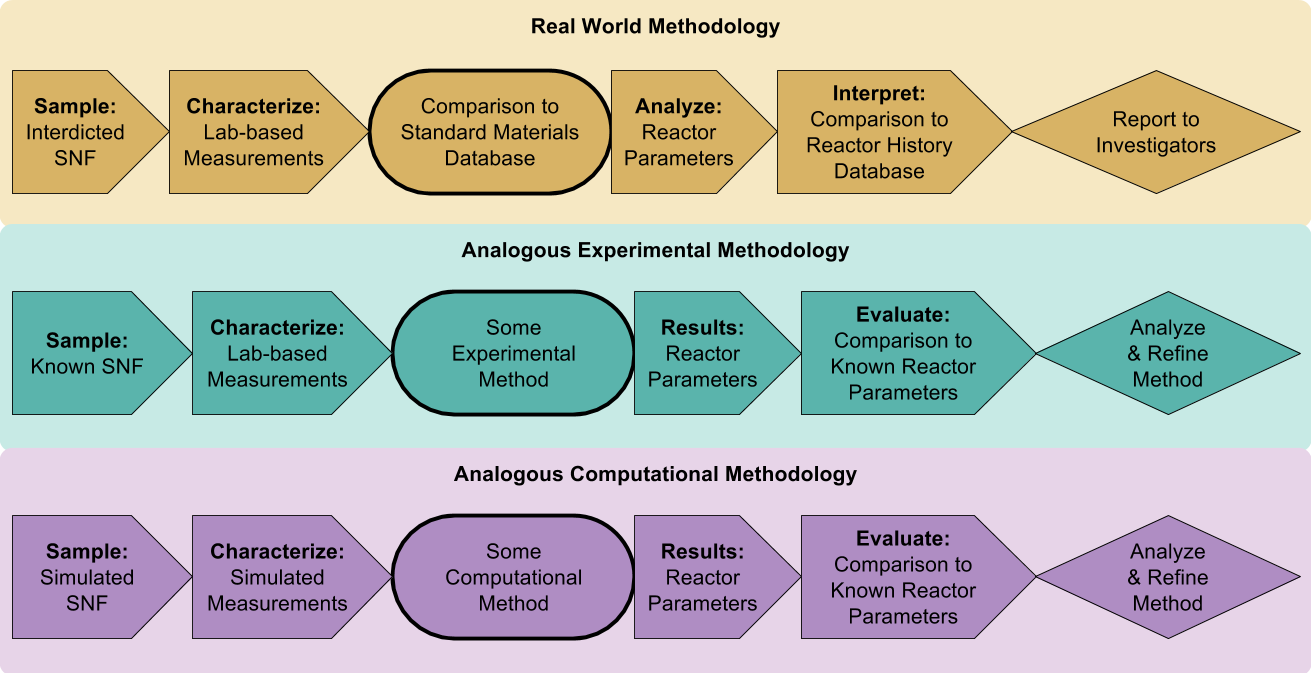
\includegraphics[width=0.9\textwidth]{./figures/ForensicsWorkflows.png}
    \caption{Comparison of computational approaches to nuclear forensics research}
  \end{figure}
\end{frame}

\begin{frame}
  \frametitle{Statistical Methods}
  Need more space to explain more about ML Models giving rxtr params? 
\end{frame}

\begin{frame}
  \frametitle{Statistical Methods}
  \begin{figure}[h!]
    \centering
    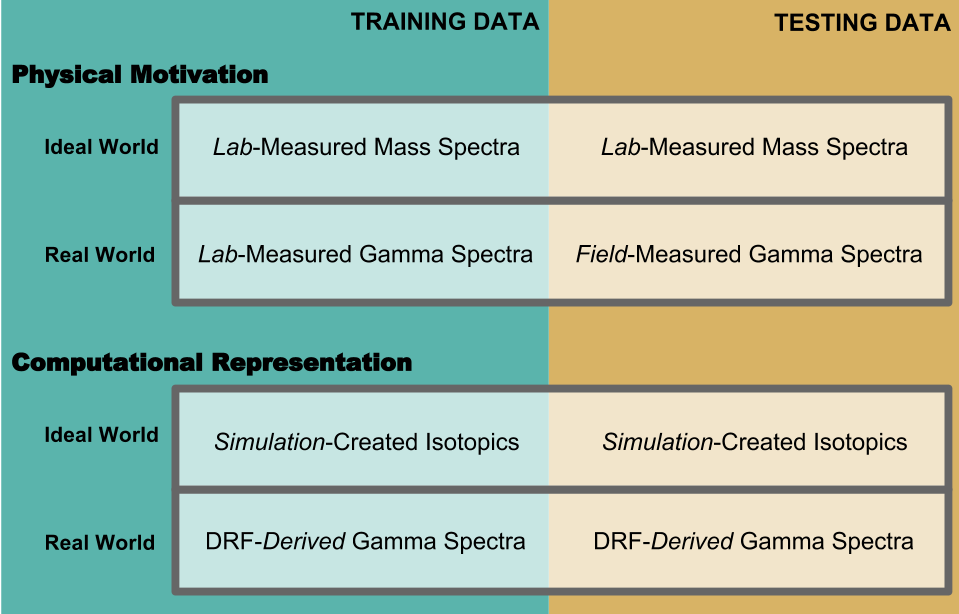
\includegraphics[width=0.9\textwidth]{./figures/proposal.png}
    \caption{The benefits of data set modularity are easily implemented in this framework}
  \end{figure}
\end{frame}

\begin{frame}
  \frametitle{Goal/Big Question}
  How does the ability to determine forensic-relevant spent nuclear fuel
  attributes using machine learning techniques degrade as less information is
  available?
\end{frame}
